%%%%%%%%%%%%%%%%%%%%%%%%%%%%%%%%%%%%%%%%%%%%%%%%%%%%%%%%%%%%%%%%%%%%%% LE RADICI
%%%%%%%%%%%%%%%%%%%%%%%%%%%%%%%%%%%%%%%%%%%%%%%%%%%%%%%%%%%%%%%%%%%%%%%%%%%%%%%%
\section{Radici}

L'idea di riprodurre con il suono anche lo spazio che lo caratterizza risale,
come altre idee ed invenzioni legate al mondo della diffusione e riproduzione
dei suoni, alla fine dell'ottocento, nell'era elettrica della rivoluzione
industriale. In quei decenni si svolgevano grandi eventi e mostre di divulgazione
tecnologica, come l'\emph{International Exposition of Electricity} tenutasi nel 1881.
Insieme a bulbi luminosi, incandescenze e batterie per l'accumulazione
dell'energia, in quel periodo ci fu spazio anche per l'idea di \emph{telefono stereo},
alla base del \emph{Théâtrophone} di Clément Ader. Per tutta la durata
dell'esposizione, ogni sera nelle sale del \emph{Grande Opera} di Parigi, veniva
suonata musica che il pubblico dell'esposizione poteva ascoltare, per alcuni
minuti, al telefono, a circa due chilometri di distanza presso il
\emph{Palais de Industrie}.

\begin{quote}
One of the most popular attractions at the \emph{Paris Electrical Exhibition} is
the nightly demonstration of the marvelous powers of the Ader telephone, by its
transmission of the singing on the stage and the music in the orchestra of the
\emph{Grand Opera} at Paris, to a suite of four rooms reserved for the purpose
in one of the galleries of the \emph{Palais de l'Industrie}. [\ldots] Certainly
nothing has ever been done before so effectually to popularize science, and to
render the masses familiar with the effect, however ignorant they may be of the
cause, of this marvelous invention, the first feeble voice of which was heard in
the \emph{Centennial Exhibition of 1876}\footnote{ \emph{Scientific American},
December 31, 1881, pages 422-423,\\ \url{https://earlyradiohistory.us/1881opr.htm}\\
Una delle attrazioni più popolari al \emph{Paris Electrical Exhibition} è la
dimostrazione notturna delle meravigliose possibilità del telefono di Ader,
che trasmette dal palco le voci e la musica dell'orchestra del \emph{Grand Opera}
di Parigi ad un gruppo di quattro sale riservate allo scopo in una delle gallerie
del \emph{Palais de l'Industrie}. [\ldots] Certamente nulla è mai stato fatto
prima in modo così efficace per divulgare la scienza e portare le masse a contatto
con l'effetto, per quanto ignoranti possano essere della causa, di questa
meravigliosa invenzione, la cui prima debole voce è stata ascoltata nella
\emph{Mostra del Centenario del 1876}.}.
\end{quote}

\begin{figure}[t]
	\centering
	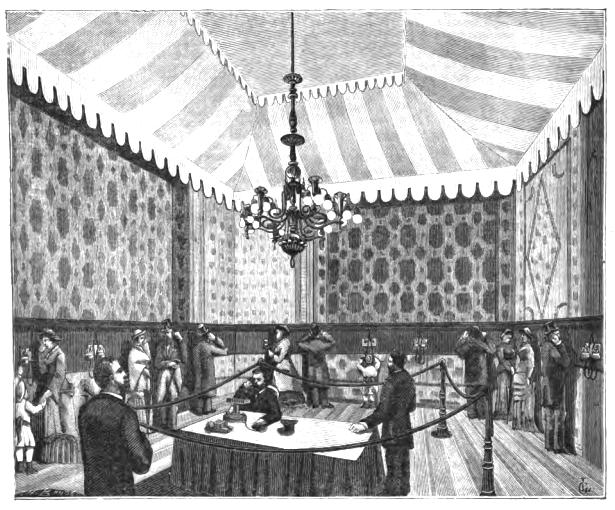
\includegraphics[width=0.99\columnwidth]{CAPITOLI/0300/IMG/1881opr4.jpg}
	\vspace{-10pt}
	\caption[]{Illustrazione della sala d'ascolto del telefono all'Esposizione di
	Parigi del 1881. Gli ascoltatori avevano i ricevitori telefonici per entrambe
	le orecchie per ascoltare il programma teatrale in stereo.}
	\label{fig:teatrophone2}
\end{figure}

Nonostante il telefono fosse un'invenzione giovanissima, al punto da pensare che
la diffusione del suono dal teatro alla sala d'ascolto avrebbe rappresentato
motivo di interesse da parte del pubblico a prescindere dalla condizione di
ascolto, Ader aggiunse l'idea di esperienza che, attraverso i concetti di
binauralità e stereofonia, ebbe un impatto incredibile sul pubblico. L'articolo
comparso su \emph{L'Electricien} in cui si descrive il funzionamento
dell'invenzione fu firmato da M. Hospitaller che descrive così l'esperienza di
ascolto:

\begin{figure}[t]
	\centering
	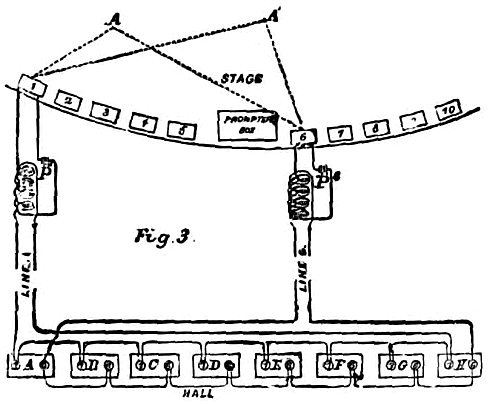
\includegraphics[width=0.99\columnwidth]{CAPITOLI/0300/IMG/1881opr2.jpg}
	\vspace{-10pt}
	\caption[]{Disposizione dei trasduttori sul palco e collegamento alle due linee
	telefoniche. Ogni ascoltatore è posizionata di fronte ad una coppia di telefoni
	i quali ricevono il segnale da due trasduttori distinti posizionati sul palco.
	Questi trasduttori sono raggruppati in coppie forniscono segnale a sedici
	telefoni, accoppiati per otto ascoltatori.}
	\label{fig:teatrophone1}
\end{figure}

\begin{quote}
We will now consider the new acoustic effect which Mr. Ader has discovered, and
applied for the first time in the telephonic transmission at the Electrical
Exhibition. Every one who has been fortunate enough to hear the telephones at
the Palais de l'Industrie has remarked that, in listening with both ears at the
two telephones, the sound takes a special character of relief and localization
which a single receiver cannot produce. [\ldots] As soon as the experiment
commences the singers place themselves, in the mind of the listener, at a fixed
distance, some to the right and others to the left. It is easy to follow their
movements, and to indicate exactly, each time that they change their position,
the imaginary distance at which they appear to be. [\ldots] This phenomenon is
very curious, it approximates to the theory of binauriclar auduition, and has
never been applied, we believe, before to produce this remarkable illusion to
which may almost be given the name of auditive perspective. [\ldots] In order
to realize it, we may recall the stereoscope, which allows us to see objects in
their natural relief\footnote{
\emph{Scientific American}, December 31, 1881, pages 422-423,\\
\url{https://earlyradiohistory.us/1881opr.htm} \\
Considereremo ora il nuovo effetto acustico che il signor Ader ha scoperto e
applicato per la prima volta nella trasmissione telefonica all'esposizione
elettrica. Tutti coloro che hanno avuto la fortuna di ascoltare i telefoni al
\emph{Palais de l'Industrie} hanno osservato che, ascoltando con entrambe le
orecchie ai due telefoni, il suono assume un carattere speciale di meraviglia e
localizzazione, cosa che un singolo ricevitore non può produrre. [\ldots] Non
appena inizia l'esperimento, i cantanti si posizionano, nella mente
dell'ascoltatore, a una distanza fissa, alcuni a destra e altri a sinistra. È
facile seguire i loro movimenti e indicare esattamente, ogni volta che cambiano
posizione, la distanza immaginaria alla quale sembrano essere. [\ldots] Questo
fenomeno è molto curioso, si avvicina alla teoria dell'audizione biauricolare che
crediamo non sia mai stato applicato prima di produrre questa straordinaria
illusione, a cui potrebbe essere dato il nome di prospettiva auditiva. [\ldots]
Per realizzarlo, possiamo ricordare lo stereoscopio, che ci consente di vedere
gli oggetti nel loro rilievo naturale.}.
\end{quote}

Tra le varie definizioni di stereofonia il termine è inoltre usato per indicare
la parte dell’acustica fisiologica che si occupa del fenomeno dell'ascolto
biauricolare del sistema uditivo. Tale fenomeno conferisce alla percezione umana
il potere localizzatore, cioè la capacità, dovuta al lavoro congiunto dei due
sistemi auricolari separati ed al sistema nervoso centrale, di determinare la
direzione di provenienza di un suono. In tal senso, esiste in acustica
fisiologica la definizione di monofonia in qualità di condizione anomala del
sistema percettivo, caratterizzata dalla mancanza degli elementi necessari a
individuare i caratteri spaziali dei suoni stessi, come per esempio quella
ottenuta con un solo orecchio.

La percezione dei caratteri spazio-temporali dei suoni, in particolare della
loro direzione di provenienza e della loro relazione con lo spazio che
attraversano, definiscono i tratti essenziali della stereofonia, in relazione
all'udito, in virtù dell’audizione biauricolare (o binaurale).

\begin{quote}
When recording music considerable trouble is experienced with the unpleasant
effects produced by echoes wich in the normal way would not be noticed by anyone
listening in the room in which the performance is taking place.
An observer in the room is listening with two ears, so that echoes reach him
with the directional significance which he associates with the music performed
in such room. He therefore discount these echoes and psychologically focuses
his attention on the source of the sound. When the music is reproduced through
a single channel the echoes arrive from the same direction as the direct sound
so that confusion results. [\ldots] Human ability to determine the direction
from which sound arrives is due to binaural hearing, the brain being able to
detect differences between sound received by the two ears from the same source
and thus to determine angular directions from which various sounds
arrive\footnote{[\cite{ab58}] - Quando si registra musica acustica, si riscontrano
notevoli problemi a causa degli effetti indesiderati prodotti dalle riflessioni
acustiche dell'ambiente, che nell'ascolto normale non vengono notati dagli
ascoltatori nella stanza in cui si svolge l'esibizione.
Un osservatore nella stanza sta ascoltando con due orecchie, in
modo che gli echi lo raggiungano con il significato direzionale che associa alla
musica eseguita in quella stanza. Pertanto, non tiene conto di questi echi e
focalizza psicologicamente la sua attenzione sulla fonte del suono. Quando la
musica viene riprodotta attraverso un singolo canale, gli echi arrivano dalla
stessa direzione del suono diretto, in modo da creare confusione. [...] La
capacità umana di determinare la direzione da cui proviene il suono è dovuta
all'udito binaurale, il cervello è in grado di rilevare le differenze tra il
suono ricevuto dalle due orecchie dalla stessa fonte e quindi di determinare le
direzioni angolari da cui provengono i vari suoni.}.
\end{quote}

È con queste parole che \adb~ nel 1931 descriveva i fondamenti delle conoscenze
in termini di percezione dei suoni e di come questi venivano utilizzati per definire
criteri tecnologici adeguati per la riproduzione dei suni. Ed è per questo che
in maniera piuttosto discreta intitola testo del brevetto che ha dato la nascita
commerciale e tecnologica alla stereofonia \emph{Miglioramenti in, ed in relazione,
ai sistemi di trasmissione del suono, registrazione del suono e riproduzione del suono}.
Genrico, inglese, la binauralità dell'ascolto umano è la prima affermazione di
Blumlein: “\emph{un osservatore nella stanza sta ascoltando con due orecchie}”.
Come questa condizione di ascolto si evolva nel tempo è la peculiarità della
stereofonia.

Il documento presenta diverse tecniche stereofoniche di microfonazione, di
incisione del disco e di trasmissione radio. La domanda fu presentata nel
dicembre 1931 ed approvata nel giugno 1933. Nel testo fa riferimento al cinema,
consapevole della necessità di migliorare la resa della registrazione sonora
in situazioni di “realismo”.

\emph{Una voce in una piccola stanza riverberante è una condizione d'ascolto che
rispetti qualità di stereofonia?}

In funzione di dei riferimenti storici e delle descrizioni fatte finora, la
risposta è chiaramente affermativa. Anche con un solo oggetto sonoro, una sola
voce, in una piccola stanza, siamo in presenza di un fenomeno acustico
stereofonico, percepito bianuralmente. Su questa condizione Blumlein presenta
le basi teoriche e tecnologiche della stereofonia, nel brevetto in cui ne
rende i concetti fondamentali, solidi, stabili nel tempo e nello spazio delle parole.

\vfill\null

\begin{figure}[bh]
\begin{bio}[Alan Dower Blumlein]
	Nato il 29 giugno 1903 a Londra, Deceduto il 7 giugno 1942 a Herefordshire,
	Inghilterra, fu ingegnere elettronico presso EMI, per la quale pubblicò brevetti
	per le sue numerose invenzioni nel campo delle telecomunicazioni soprattutto in
	relazione alle tecnologie di registrazione, trasmissione e diffusione del suono.
	Ottiene, nella sua breve carriera, 128 brevetti, motivo per cui è considerato
	uno dei più importanti ingegneri e inventori del suo tempo. Morì durante la
	seconda guerra mondiale all'età di 38 anni, durante un test militare segreto del
	sistema radar H2S allora in fase di sviluppo, a bordo del bombardiere Halifax
	su cui stava volando. Tra le numerose invenzioni legate al nome di Blumlein
	quelle legate alla Stereofonia stravolsero completamente il mondo della
	fruizione pubblica del suono. Le sue prime note sull'argomento risalgono al 25
	settembre 1931 e il suo brevetto aveva il titolo “Miglioramenti ai, ed in
	relazione ai, sistemi di trasmissione, registrazione e riproduzione del suono”.
	La domanda di brevetto fu del 14 dicembre 1931 ed la concessione fu dell
	14 giugno 1933, brevetto britannico numero 394.325.
\end{bio}
\end{figure}

% \vfill\null
%
% %------------------------- APPROFONDIMENTO
% %\begin{figure}[th]
% \begin{table}[ht]
% \footnotesize
% \begin{tabular}{L{.969\textwidth}}%
% \toprule
% 	\textbf{Michael Antony Gerzon}\\
% \midrule
% Nato il 4 dicembre 1945, deceduto il 6 maggio 1996. Matematico, all'università
% aveva già un forte interesse sia per la teoria che per la pratica della
% registrazione, che condivideva con alcuni colleghi studenti tra cui Peter Craven
% (i due furono in seguito i co-inventori del microfono \emph{Soundfield} e
% collaborarono a molti altri progetti). Dagli nei primi anni settanta sviluppa la
% tecnologia \emph{Ambisonics}, che può essere descritta come un completamento teorico
% e pratico del lavoro svolto da Alan Blumlein nel campo del suono stereofonico.
% Gerzon morì nel 1996 per complicazioni dovute a un grave attacco d'asma. \\
% \bottomrule
% \end{tabular}
% \end{table}
% %\end{figure}
% %------------------------- APPROFONDIMENTO
